% -*- TeX:Soft -*-
\documentclass[11pt]{article}
\usepackage{amsmath}
\usepackage{graphicx}
\usepackage{amsfonts}
\usepackage{listings}
\usepackage{optprog}
\usepackage{color}
\usepackage{makeidx}
\usepackage[latin9]{inputenc}
\usepackage{flafter}% Causes floats to show AFTER cited
%\usepackage{hyperref} %clean files .aux, .toc, etc before using hyperref.
\usepackage{epstopdf}
\usepackage{bm}
\usepackage[breaklinks]{hyperref}
\usepackage{xspace}

\definecolor{darkgreen}{rgb}{0.00,0.50,0.25}

\title{jPhase User's Guide}
\author{Juan F. P�rez \hspace{1.3cm} Germ\'an Ria\~no\\
%Universidad de Los Andes\\
\footnotesize{fern-per@uniandes.edu.co \hspace{0.6cm} griano@uniandes.edu.co}\\
  Centro de Optimizaci{\'o}n y Probabilidad Aplicada (COPA)\\
  Departamento de Ingenier{\'\i}a Industrial\\
  Universidad de los Andes\\
  Bogot�, Colombia}
\date{}

\newcommand {\cA}{\ensuremath \mathcal{A}}
\newcommand {\cS}{\ensuremath \mathcal{S}}
\newcommand {\lil}{\lstinline}
\DeclareMathOperator*{\argmax}{argmax}
\newtheorem{rem}{Remark}

%\lstset{
%  basicstyle=\small,
%  language=java,
%  frame=single,
%  tabsize=2,
%  showstringspaces=false,
%  morecomment=[s][\color{darkgreen}]{/*}{*/},
%  morecomment=[l][\color{darkgreen}]{//},
%  morecomment=[s][\color{blue}]{/**}{*/},
%  morestring=[d][\color{blue}]{"}
%}
\definecolor{purple}{rgb}{0.40,0.00,0.45}
\definecolor{green}{rgb}{0.00,0.25,0.00}
\lstset{
    basicstyle=\small,
    language=java,
    frame=single,
    keywordstyle=\color{purple}\bfseries,
    morestring=[d][\color{blue}]{"},
}

\newcommand{\lstinclude}[1]{
  %\lstset{title={\large{File \lstinline[basicstyle=\large\ttfamily]|#1|}}
   %       }
  \lstinputlisting{#1}
  %\addcontentsline{toc}{subsubsection}{File \lstinline|#1|}
  \lstset{title={}}
}
\lstnewenvironment{lstverbatim}{\lstset{title=Output}}{}





%\textcolor[rgb]{0.00,0.50,0.25}{}
%\newcommand{\lstinclude}[1]{
%  \lstset{title={\Large{File #1}},basicstyle=\small}
%  \lstinputlisting{../../examples/jmdp/#1}
%}


%\lstset{language=[AspectJ]Java, basicstyle=\small,
%commentstyle=\footnotesize,
%tabsize=2,frame=single, breakautoindent=true}

\setlength{\oddsidemargin}{0pt} \setlength{\textwidth}{6.5in}
\setlength{\marginparsep}{0pt} \addtolength{\voffset}{-0.8cm}


\addtolength{\textheight}{2.0in}
\makeindex


\newcommand{\jPhase}{\textbf{jPhase}\xspace}
\newcommand{\jPhaseFit}{\textbf{jPhaseFit}\xspace}
\newcommand{\jPhaseGen}{\textbf{jPhaseGenerator}\xspace}
\newcommand{\DiscPhaseVar}{\texttt{Disc\-Phase\-Var}}
\newcommand{\ContPhasevar}{\texttt{Cont\-Phase\-Var}}
\newcommand{\balpha}{\boldsymbol{\alpha}}
\newcommand{\bbeta}{\boldsymbol{\beta}}
\newcommand{\bgamma}{\boldsymbol{\gamma}}
\newcommand{\bA}{\boldsymbol{A}}
\newcommand{\bB}{\boldsymbol{B}}
\newcommand{\bC}{\boldsymbol{C}}
\newcommand{\bQ}{\boldsymbol{Q}}
\newcommand{\ba}{\boldsymbol{a}}
\newcommand{\bb}{\boldsymbol{b}}
\newcommand{\bc}{\boldsymbol{c}}
\newcommand{\one}{\boldsymbol{1}}
\newcommand{\zero}{\boldsymbol{0}} 



\begin{document}
%\renewcommand{\includegraphics}[2][]{\framebox{File #2.eps Missing!}}

\maketitle
\tableofcontents
\newpage

\section*{Introduction}

Phase-Type (PH) distributions are a powerful tool in stochastic models of real systems. \jPhase \cite{pere.rian:jphase} is a Java-based framework that allows the representation of PH distributions through computational objects. The developed structure induces a formal representation of a Phase-type distribution and a set of properties that it should have.
In this Manual, we illustrate the use of \jPhase through several examples that are included in each section. This document is organized as follows: the first section gives an introductory background in PH distributions. Section 2 shows how the core module \jPhase if structured and gives some examples. Sections 3 and 4 illustrate the structure of the packages \jPhaseFit and \jPhaseGen, and also give several examples of how to use the services provided by the package. More examples and applications for stochastic modeling with \textbf{jMarkov} can be found in the release that can be downloaded from \texttt{copa.uniandes.edu.co}.

\section{Phase-Type Distributions}
\label{sc:PH}
 
In this section, we review the definition and some properties of PH distributions. We follow the treatment presented in \cite{neut81} and \cite{lato.rama99}, and therefore, we do not include proofs in this section since the interested reader can find them in those books.

\subsection{Continuous Phase-Type Distributions}

A Continuous Phase-Type distribution can be defined as the time until absorption in a Continuous Markov Chain, with one absorbing state and all others transient. The generator matrix of that process can be written as:
\begin{gather*}
\bf{Q}=
\begin{bmatrix}
  0          & \bf{0} \\
  \bf{a}     & \bf{A}
\end{bmatrix},
\end{gather*}
\noindent where the first entry in the state space represents the absorbing state. As the sum of the elements on each row must equal zero, {\bf a} is determined by
\[\bf{a}=-\bf{A1},\]
where {\bf 1} is a column vector of ones. In order to completely determine the process, the initial probability distribution is defined and can be partitioned in the same way of the generator matrix
\[
\begin{bmatrix}
  \alpha_0  & {\bm \alpha}
\end{bmatrix},
\]
where $\alpha_0$ is the probability of starting the process in the state $0$, and the sum of all the components in the vector must be equal to 1. Therefore, $\alpha_0$ is determined by the following relationship 
\[ \alpha_0 = 1 - \bm{\alpha1}.\]

In this way, the distribution of a Continuous Phase-Type variable $X$ is completely determined by the parameters $({\bm \alpha, A})$, and its cumulative distribution function (CDF) is
\[F(x)=1-{\bm \alpha} e^{{\bf A}x} {\bf 1}, \quad x \geq 0,\]
which has a clear connection to the well known exponential distribution. Furthermore, if there is just one transient phase with associate rate $\lambda$ and it is selected with probability one, then the distribution is exactly the exponential case. From the previous expression, the probability density function (PDF) of the continuous part can be computed as 
\[f(x)={\bm \alpha} e^{{\bf A}x} {\bf a}, \quad x > 0.\]
And similarly, the Laplace-Stieltjes transform of $F(\cdot)$, is given by
\[\alpha_0 + {\bm \alpha} (s{\bf I}-{\bf A})^{-1} {\bf a}, \quad Re(s) \geq 0,\]
from which, the non-centered moments can be calculated as
\[E[X^k]=k! {\bm \alpha} (-{\bf A}^{-1})^k {\bf 1}, \quad k \geq 1.\]


\subsection{Discrete Phase-Type Distributions}
A Discrete Phase-Type distribution can be seen as an analogous case to the continuous distribution. In this case, the distribution can be defined as the number of steps until absorption in a Discrete Markov Chain, with one absorbing state and all other transient. The transition probability matrix of that process may be defined as:
\begin{gather*}
\bf{P}=
\begin{bmatrix}
  1          & \bf{0} \\
  \bf{a}     & \bf{A}
\end{bmatrix},
\end{gather*}
where the first row in the matrix represents the absorbing state. As the sum of the elements in every row of the matrix must equal one (in order to be a probability mass function), {\bf a} is determined by:
\[\bf{a}={\bf 1}-\bf{A1}.\]
Similarly, the initial probability distribution is defined as
\[
\begin{bmatrix}
  \alpha_0  & {\bm \alpha}
\end{bmatrix},
\]
\noindent where $\alpha_0=1-\bm{\alpha1}$ is the probability of starting the process in the absorbing state, i.e. the number of steps in that case would be equal to zero. As before, the distribution of a discrete Phase-Type variable $X$ is completely determined by the parameters $(\alpha, A)$ and its probability mass function is defined as
\begin{gather*}
P\{X=k\}=\begin{cases} \alpha_0 & ,k=0\\
{\bm \alpha} {\bf A}^k{\bf a} & ,k \geq 1
\end{cases}
\end{gather*}

This last definition makes natural the definition of the cumulative probability function of the discrete Phase-Type variable

\[P\{X \leq k\}= 1 - {\bm \alpha} {\bf A}^k {\bf 1}, \quad k \geq 0.\]
Also, the generating function can be calculated as
\[ \alpha_0 + z{\bm \alpha} ({\bf I}-z{\bf A})^{-1} {\bf a}, \quad |z| \leq 1.\]
from which, the factorial moments of the distribution can be computed
\[E[X(X-1)\dots(X-k+1)]=k! {\bm \alpha} ({\bf I} - {\bf A})^{-k} {\bf A}^{k-1} {\bf 1}, \quad k \geq 1.\]






\subsection{Closure Properties}

An important issue of Phase-Type distributions is that they are closed under some operations, which can be useful in the analysis of some systems. The following closure properties are valid for both discrete and continuous distributions.

\begin{enumerate}
\item {\bf Convolution of a finite number of Phase-Type distributions}\\%
If $X \sim PH({\bm \alpha},\bf{A})$ and $Y \sim PH({\bm \beta}, \bf{B})$ (independent of $X$), with $n$ and $m$ phases respectively, then the convolution is $PH({\bm \gamma}, \bf{C})$ with $m+n$ phases and 
\begin{align*}
{\bm \gamma}&=[{\bm \alpha}, \alpha_0 {\bm \beta}]&\text{and}&&
{\bf C}&=	\begin{bmatrix}
			  {\bf A}  & {\bf a }{\bm \beta} \\
			  {\bf 0}  & {\bf B}
		\end{bmatrix}.
\end{align*}
	
\item {\bf Convex mixture of a finite number of Phase-Type distributions}\\%
If $X \sim PH({\bm \alpha},\bf{A})$ and $Y \sim PH({\bm \beta}, \bf{B})$ (independent of $X$), with $n$ and $m$ phases respectively, and distribution functions $F(\cdot)$ and $G(\cdot)$. Then, the convex mixture $\theta F(\cdot) + (1-\theta)G(\cdot)$, with $0\leq \theta \leq 1$, has representation $PH({\bm \gamma}, \bf{C})$ with $m+n$ phases, where 
\begin{align*}
{\bm \gamma}&=[\theta {\bm \alpha}, (1-\theta) {\bm \beta}]&\text{and}&&
{\bf C}&=	\begin{bmatrix}
			  {\bf A}  & {\bf 0} \\
			  {\bf 0}  & {\bf B}
		\end{bmatrix}.
\end{align*}

\item {\bf Convolution of a discrete Phase-Type number of Phase-Type distributions}\\%
If $X_i$ are i.i.d. continuous $PH({\bm \alpha},\bf{A})$ and $N$ is a discrete $PH({\bm \beta}, \bf{B})$, then  $\sum_{k=0}^{N}X_i$ is $PH({\bm \gamma}, \bf{C})$, with
\begin{align*}
{\bm \gamma}& = {\bm \alpha} \otimes {\bm \beta}&\text{and}&&
{\bf C}&=	{\bf A} \otimes {\bf I} + {\bf a }{\bm \alpha} \otimes {\bf B}.
\end{align*}

The function $\otimes$ denotes the Kronecker product and $\oplus$ the Kronecker sum. \footnote{
The Kronecker product of matrices ${\bf A}$ and ${\bf B}$ is defined as 
\[{\bf A} \otimes {\bf B} = 
\begin{bmatrix}
	  a_{11}{\bf B} & a_{12}{\bf B} &\dots	& a_{1n}{\bf B}\\
	  a_{21}{\bf B} & a_{22}{\bf B} &\dots	& a_{2n}{\bf B}\\
	  \vdots				&	\vdots				&\ddots	&\vdots			\\
	  a_{m1}{\bf B} & a_{m2}{\bf B} &\dots	& a_{mn}{\bf B}
\end{bmatrix}\]
And the Kronecker sum of matrices ${\bf A}$ and ${\bf B}$ is defined as ${\bf A} \oplus {\bf B} = {\bf A}\otimes {\bf I} + {\bf I}\otimes {\bf B}$.}


As the geometric distribution is a particular case of Discrete Phase-Type distributions, this property also holds for the geometric case. If $X_i$ are i.i.d. continuous $PH({\bm \alpha},\bf{A})$ and $N$ follows a geometric distribution with parameter $p$, then $\sum_{k=0}^{N}X_i$ is $PH({\bm \gamma}, \bf{C})$, with
\begin{align*}
{\bm \gamma}& = {\bm \alpha}&\text{and}&&
{\bf C}&=	{\bf A} + (1-p){\bf a}{\bm \alpha}.
\end{align*}



\item {\bf The minimum of a set of Phase-Type distributions}\\%
If $X \sim PH({\bm \alpha},\bf{A})$ and $Y \sim PH({\bm \beta}, \bf{B})$ (independent of $X$), with $n$ and $m$ phases respectively, then $min(X,Y) \sim PH({\bm \gamma}, \bf{C})$ with $mn$ phases and  
\begin{gather*}
{\bm \gamma} = {\bm \alpha} \otimes {\bm \beta}.
\end{gather*}
In this case, the matrix $C$ has a different definition if the process is discrete or continuous. In the discrete case, the resulting probability transition matrix is given by
\begin{gather*}
{\bf C}=	{\bf A} \otimes {\bf B}.
\end{gather*}
For the continuous case, the generator matrix is given by
\begin{gather*}
{\bf C}=	{\bf A} \oplus {\bf B}.
\end{gather*}


\item {\bf The maximum of a set of Phase-Type distributions}\\%
If $X \sim PH({\bm \alpha},\bf{A})$ and $Y \sim PH({\bm \beta}, \bf{B})$ (independent of $X$), with $n$ and $m$ phases respectively, then $max(X,Y) \sim PH({\bm \gamma}, \bf{C})$ with $mn+n+m$ phases and  
\begin{align*}
{\bm \gamma}&=[{\bm \alpha} \otimes {\bm \beta}, \beta_0{\bm \alpha}, \alpha_0{\bm \beta}]\\
{\bf C}&=	\begin{bmatrix}
			  {\bf A} \oplus {\bf B} 	& {\bf I} \otimes {\bf b}	& {\bf a} \otimes {\bf I} \\
			  {\bf 0}  								& {\bf A}									& {\bf 0}\\
			  {\bf 0}  								& {\bf 0}									& {\bf B}\\
		\end{bmatrix}.
\end{align*}
\end{enumerate}




\subsection{Further Closure Properties for Continuous Distributions \label{sc:closeContPH}}
There are some other important closure properties that only apply for the case of Continuous Phase-Type distributions, which are listed below.

\begin{enumerate}

\item {\bf Waiting time in a $M/PH/1$ queue}\\%
If $X \sim PH({\bm \alpha},\bf{A})$ is the service time distribution in a $M/G/1$ queue, then the distribution of the waiting time $W(\cdot)$ is $PH({\bm \gamma}, \bf{C})$, with
\begin{align*}
{\bm \gamma}&=(1-\rho){\bm \pi} &\text{and}&&
{\bf C}&=	{\bf A} + \rho {\bf a}{\bm \pi},
\end{align*}
\noindent where $\rho=\lambda m$ is the traffic coefficient, $\lambda$ is the arrival rate and $m$ is the expected value of the service time. ${\bm \pi}$ is the stationary probability vector of ${\bf A} + {\bf a} {\bm \alpha}$, i.e. ${\bm \pi} = ({\bm \alpha} {\bf A}^{-1}{\bf 1}){\bm \alpha}{\bf A}^{-1}$.


\item {\bf Residual time distribution}\\%
If $X \sim PH({\bm \alpha},\bf{A})$, then the residual time distribution \[G(x) = \text{P}(X - \tau \leq x | X > \tau)\] has representation $PH({\bm \gamma}, \bf{C})$, with
\begin{gather*}
{\bm \gamma} = \frac{1}{1-F(\tau)} \, {\bm \alpha }e^{{\bf A}\tau} .
\end{gather*}


\item {\bf Equilibrium Residual time distribution}\\%
If $X \sim PH({\bm \alpha},\bf{A})$, then the equilibrium residual time distribution \[G(x) = \frac{1}{E[X]}\int_0^x(1 - F(u))du,\]  has representation $PH({\bm \pi}, \bf{A})$, where ${\bm \pi}$ has the same meaning as stated above.


\item {\bf Termination time of a Phase-Type process with Phase-Type failures \cite{neut92}}\\%
Consider a process where the service time is determined by Phase-Type distribution with $m$ phases and representation $PH({\bm \alpha},\bf{A})$, and it is subject to failures that occur according to a Poisson process with rate $\lambda$. If the duration of the failure is $PH({\bm \beta}, \bf{B})$ with $n$ phases, then the total completion time has distribution $G(\cdot)$ with representation $PH({\bm \gamma}, \bf{C})$. Two different cases must be differentiated: if the service must be restarted after the failure, or if the task can begin from the point where it was left before the failure. In the first case, the resulting distribution has $m+n$ phases and
\begin{align*}
{\bm \gamma}& = [{\bm \alpha}, {\bf 0}]&\text{and}&&
{\bf C}&=	\begin{bmatrix}
			  {\bf A}-\mu{\bf I} 	& \mu{\bf 1}{\bm \beta} \\
			  {\bf b}{\bm \alpha} & {\bf B}
		\end{bmatrix}.
\end{align*}
\noindent In the second case, the representation has $m+mn$ phases and
\end{enumerate}
\begin{align*}
{\bm \gamma}& = [{\bm \alpha}, {\bf 0}]&\text{and}&&
{\bf C}&=	\begin{bmatrix}
			  {\bf A}-\mu{\bf I} 		& \mu{\bf I}\otimes{\bm \beta} \\
			  {\bf I}\otimes{\bf b} & {\bf I}\otimes{\bf B}
		\end{bmatrix}.
\end{align*}


The Continuous and Discrete Phase-Type distributions have the important property of being dense in $[0,\infty)$ and the non-negative integers, respectively (the proof of this property can be found in \cite{fang99}). This implies that any distribution with support on those sets can be approximated by a Phase-Type distribution with the appropriate number of phases and parameters ${\bm \alpha}$ and {\bf A}. 

\subsection{Phase-Type Random Variates Generation}
\label{sc:genPH}

In many large applications, simulation is the appropriate tool to model the system because of the complex relations between different stochastic variables. This makes that a random number generator become an important tool to model a wide range of non-deterministic systems. Neuts and Pagano \cite{neut.paga81} developed two similar algorithms to generate random variates from discrete and continuous Phase-Type distributions. These algorithms are supported on the alias method \cite{law.kelt00} to generate variates from discrete distributions in order to simulate the process of selecting an initial state and then jump to the next one according to random vectors.


\subsection{Fitting Algorithms}
In the last twenty years, the problem of fitting the parameters of a Phase-Type distribution has received great attention from the applied probability community. These different approaches can be classified in two major groups: maximum likelihood methods and moment matching techniques, as noted in \cite{lang.arth96}. Nevertheless, almost all the algorithms designed for this task have an important characteristic in common: they reduce the set of distributions to be fitted, from the whole Phase-Type set to a special subset. In section \ref{sc:fitter}, those algorithms included in the computational package will be revisited and further explained. 





%\newpage
\section{\jPhase: the object-oriented Framework}
\label{sc:jphase}

\subsection{General Structure}

The \texttt{jPhase} package is supported on a set of interfaces, abstract classes and implementing classes. The interfaces determine the characteristics of an object and have no implementation of any method. As can be seen in the simple Class Diagram of Figure \ref{fig:phaseVar}, there are three interfaces in the jPhase package: \texttt{PhaseVar}, \texttt{Cont\-Phase\-Var},  and \texttt{Disc\-Phase\-Var}. These interfaces determine the behavior of a PH distribution in both the continuous and discrete cases.

\begin{figure*}[ht] \centering
    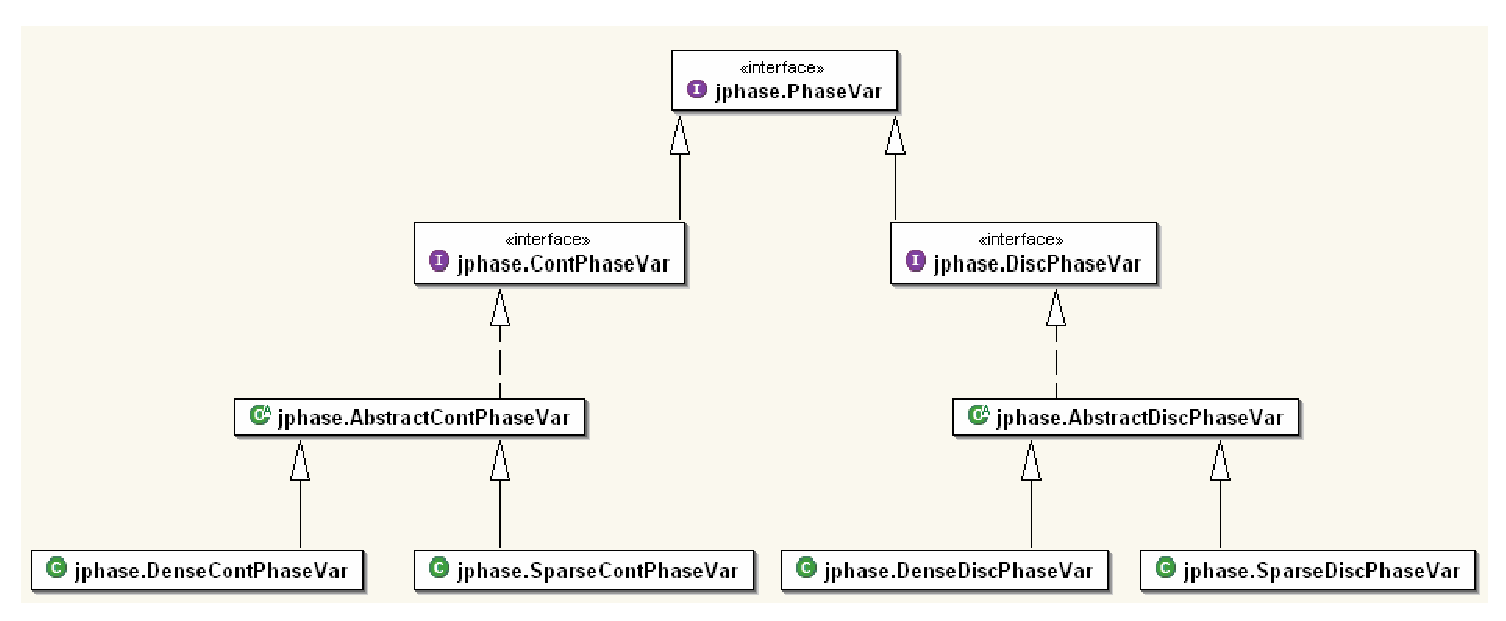
\includegraphics[width=15cm, height=5.5cm]{figs/jphase}% height=1.5in
    \caption{Simple \jPhase Package Class Diagram}
    \label{fig:phaseVar}
\end{figure*}

The abstract classes \texttt{Abstract\-Cont\-Phase\-Var} and \texttt{Abstract\-Disc\-Phase\-Var} implements the corresponding interface (discrete or continuous), in order to develop some of the methods determined by the interfaces. Finally, the implementing classes extends the corresponding abstract class, and thus they make use of the already implemented methods. These methods are useful for any user that wants to develop his own implementing class, because he does not need to get worried about the whole set of distribution properties, but only needs to implement a little set of simple methods. In the next sections, the properties of these interfaces, abstract and implementing classes will be explained.

\subsection{Interfaces}
As it was said above, the jPhase package consists of three interfaces, that determine the behavior of any PH distribution as shown next.
\begin{itemize}
	\item \texttt{PhaseVar}\\ This interface defines properties that are common to both discrete and continuous Phase-type distributions. Since this is the core interface in the framework, it has the major quantity of methods and all other interfaces ans classes have fewer. The methods that the interface force to implement for any distribution can be divided in three groups: access, moments and distribution methods. 
	
		
	\item \texttt{Disc\-Phase\-Var} and \texttt{Cont\-Phase\-Var}\\This interfaces determine some of the closure properties valid for discrete and continuous PH variables, as those discussed in section \ref{sc:PH}. The methods defined by each one of this interfaces can be partitioned in two groups: distribution and closure methods. The closure properties can only be defined at this level because each one of the discrete and continuous sets are closed under these properties, but not the whole set of PH distributions.

\end{itemize}


\subsection{Abstract Classes}

As shown in Figure \ref{fig:phaseVar}, the \texttt{Cont\-Phase\-Var} interface is implemented by the abstract class \texttt{Abs\-tract\-Cont\-Phase\-Var}, which implements almost all the methods defined by \texttt{Phase\-Var} and \texttt{Cont\-Phase\-Var}. In particular, none of the methods implemented by this class depends on the formal representation of the matrices and vectors involved. This means that all the operations are executed using solvers and preconditioners that apply for both sparse and dense representations of matrices and vectors. Moreover the probably most difficult routines are solved by this abstract class, such as the computation of the probability density function, that implies the use of uniformization methods for solve a set of differential equations\cite{lato.rama99}. The same arguments apply for the abstract class \texttt{Abs\-tract\-Disc\-Phase\-Var}, that implements the interface \texttt{Disc\-Phase\-Var}.

This way, the only methods that the user must implement when developing an implementing class are: \texttt{get\-Ma\-trix} and \texttt{set\-Ma\-trix}; \texttt{get\-Vec\-tor} and \texttt{set\-Vec\-tor}; \texttt{new\-Var} and \texttt{copy}. 

As can be seen, this methods depend on the particular representation of the distribution, e.g. if the matrix is represented by a particular sparse pattern, then the only one class of matrices that can be set must have the same pattern. Since jPhase is built over the Matrix Toolkit for Java (MTJ) library \cite{heim05}, the user could develop his own representations over those offered by MTJ. Also the \texttt{newVar} and \texttt{copy} methods must return a variable that belongs to the same class of the original one. The implementing classes explained in the next section are themselves examples of classes that extend the abstract ones.


\subsection{Implementing Classes}

The developed implementing classes are those that a final user will utilize. They have been designed as general PH representations for the continuous and discrete cases, and with dense and sparse storage. The \texttt{Dense\-Cont\-Phase\-Var} and \texttt{Dense\-Disc\-Phase\-Var} classes represent continuous and discrete PH distributions, using the \texttt{Dense\-Matrix} and \texttt{Dense\-Vector} classes defined by MTJ \cite{heim05}. These classes are useful for many applications, where the number of phases is not large and the memory is not a problem. They also have constructors for many simple distributions such as exponential or Erlang in the continuous case, and geometric or negative binomial in the discrete case.

Nevertheless, the use of matrices with dense representation can be a problem because of the large number of phases. The \texttt{Sparse\-Cont\-Phase\-Var} and \texttt{Sparse\-Disc\-Phase\-Var} classes are built over the \texttt{Flex\-Comp\-Row\-Matrix} and \texttt{Sparse\-Vector} MTJ classes, which give a good alternative when the number of phases is large but the number of entries is little relative to the total number of $n^2$ entries. It is important to note that the \texttt{Flex\-Comp\-Row\-Matrix} allows a flexible sparse pattern stored by rows, that makes of this class a general sparse representation. Other specific representation could be developed by using a particular sparse pattern, e.g. upper-diagonal matrices.




\subsection{\jPhase Examples}
\label{sc:exam}
In this section, the use of \jPhase is illustrated through relevant examples. All of these examples should be included in a class with a main class that calls them to be executed. In Figure \ref{fig:ex1}, two PH variables: $V_1$ is a exponential variable with parameter $\lambda=3$, and $V_2$ is an Erlang variable with parameters $\lambda=1.5$ and $k=2$. Once this is done, a third variable ($V_3$) is created as the maximum between $V_1$ and $V_2$. Finally, the probability that $V_3$ takes a value not greater than $2.0$ is computed through the cumulative density function. This value is printed and is shown in Figure \ref{fig:resEx1}.
\begin{figure}[htbp]
	\centering
	\lstinclude{figs/example1.java}
	\caption{\jPhase: Example 1}
	\label{fig:ex1}
\end{figure}

\begin{figure}[htbp]
	\centering
	\lstinclude{figs/resExample1.txt}
	\caption{\jPhase: Result for Example 1}
	\label{fig:resEx1}
\end{figure}




\begin{figure}[htbp]
	\centering
	\lstinclude{figs/example2.java}
	\caption{\jPhase: Example 2}
	\label{fig:ex2}
\end{figure}

\begin{figure}[htbp]
	\centering
	\lstinclude{figs/resExample2.txt}
	\caption{\jPhase: Result for Example 2}
	\label{fig:resEx2}
\end{figure}


Figure \ref{fig:ex2} shows again the creation of two particular PH variables: $V_1$ is an Erlang variable with parameters $\lambda=0.8$ and $k=3$, and $V_2$ is an Erlang variable with parameters $\lambda=1.5$ and $k=2$. Then, the variable $V_3$ is created as the sum of $V_1$ and $V_2$. This variable is printed, and the result is shown in Figure \ref{fig:resEx2}. The printed version of the variable includes the initial probability vector ${\bm \alpha}$ and the transition matrix {\bf A}, as explained in section \ref{sc:PH}.


\begin{figure}[htbp]
	\centering
	\lstinclude{figs/example3.java}
	\caption{\jPhase: Example 3}
	\label{fig:ex3}
\end{figure}

\begin{figure}[htbp]
	\centering
\lstinclude{figs/resExample3.txt}
	\caption{\jPhase: Result for Example 3}
	\label{fig:resEx3}
\end{figure}

As shown in Figure \ref{fig:ex3}, the distributions can be created from arrays of doubles, that represent the initial probability vector and the generator matrix of the transient states (as specified in section \ref{sc:PH}). Once the distributions are created, they can be manipulated through the use of closure properties, as shown in Figure \ref{fig:ex3}, where the sum of the variables $v1$ and $v2$ is calculated. The resulting variable is shown next in Figure \ref{fig:resEx3}, where the calculated variable is printed.


\begin{figure}[htbp]
	\centering
	\lstinclude{figs/example4.java}
	\caption{\jPhase: Example 4}
	\label{fig:ex4}
\end{figure}

\begin{figure}[htbp]
	\centering
	\lstinclude{figs/resExample4.txt}
	\caption{\jPhase: Result for Example 4}
	\label{fig:resEx4}
\end{figure}

Since \jPhase is built over the Matrix Toolkit for Java (MTJ) library \cite{heim05}, it is also possible to construct PH distributions from matrices and vectors defined in that library. As can be seen in Figure \ref{fig:ex4}, the matrix and the vector of the PH distribution are first built as \texttt{DenseMatrix} and \texttt{DenseVector} (MTJ objects), and then the continuous PH distribution is constructed. In this example, the distribution of the waiting time in queue is computed taking the variable $V_1$ as the service time distribution and assuming that the traffic coefficient of the M/PH/1 queue is equal to $0.5$. The resulting distribution is then printed and the output is shown in Figure \ref{fig:resEx4}.

Another way to do the former calculations is through the use of the Graphic User Interface (GUI). This can be used to build PH variables from direct input, or from a data set that can be fit the parameters of the distribution. It also allows to compute closure properties and has the capabilities to show graphically the probability density function or the cumulative probability distribution of a specified PH distribution. 


As can be seen, the developed framework is an easy way to deal with PH distributions and can be used as a supporting tool in several practical researches, where the main point is to build a probabilistic model that describes the system, and the PH distributions are an important tool to do it. Thus, the researcher can focus on the modeling issue based on the computational representation developed in this work.







%\newpage
\section{\jPhaseGen: the variates generator Module}
\label{sc:gen}

This package was developed in order to define the behavior of any PH random variates generator. This behavior is specified by the abstract class \texttt{Pha\-se\-Gene\-ra\-tor}, which is the core the package. As can be seen in Figure \ref{fig:phaseGenerator}, this abstract class is extended by the implementing classes \texttt{Neuts\-Cont\-PH\-Gene\-ra\-tor} and \texttt{Neuts\-Disc\-PH\-Gene\-ra\-tor}. Those classes implement the algorithms proposed by Neuts and Pa\-ga\-no \cite{neut.paga81}.

\begin{figure}[ht] \centering
    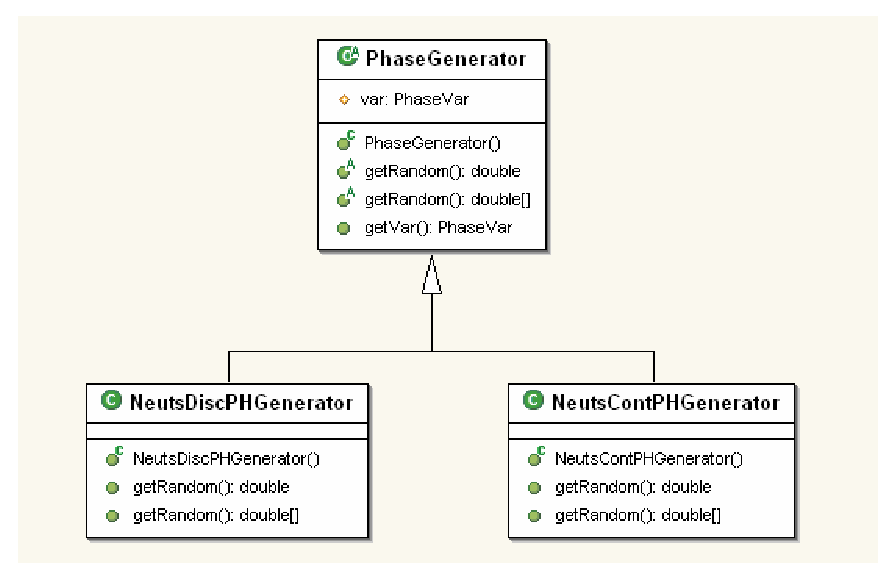
\includegraphics[width=9cm, height=5.5cm]{figs/jphasegenerator}% height=1.5in
    \caption{Simple jPhaseGenerator Package Class Diagram }
    \label{fig:phaseGenerator}
\end{figure}

\subsection{\texttt{Phase\-Generator} Interface}

This abstract class defines the basic methods that a PH random variate generator should have. The class includes an attribute, that belongs to the \texttt{PhaseVar} class, and is the distribution from which, the random variates will be generated. This distribution can only be specified in the constructor method, because the variable must be persistent in time for a particular \texttt{Phase\-Generator} object. This means that if the user wants to generate variates from another distribution, he must create a new \texttt{Phase\-Generator}.

In the constructor method, the variable is assigned and the \texttt{initialization()} method is called. It is expected that the user make use of this method in order to effectively initialize the algorithm, and then a random variate can be generated after the construction of the PhaseGenerator. Another method defined by the abstract class is \texttt{getVar()}, which always returns the PH variable that remain under the PhaseGenerator and is already implemented.

The last two methods that a PhaseGenerator must implement are \texttt{getRandom()} and \texttt{getRandom($k$)}. The first one must return a variate that follows the distribution specified at the construction, and the second must return $k$ independent variates with the same characteristic.

\subsection{Implementing Classes}
Currently, there are two implementing classes that extend the previously explained \texttt{Phase\-Gene\-ra\-tor} abstract class. These are \texttt{Neuts\-Cont\-PH\-Gene\-rator} and \texttt{Neuts\-Disc\-PH\-Gene\-rator}, which implement the methods proposed by Neuts and Pagano \cite{neut.paga81}. The first one implements the continuous case and the second the discrete one. The continuous algorithm has a first step, in which a discrete chain is biult over the continuous one, using the well-known embedded chain. Thereafter, the main algorithm (for discrete distributions) can be used for both cases.

The algorithm simulates the whole process in the chain: it first choose an initial state from the distribution given by the initial probability vector; then it selects a next state to visit using the discrete distribution associated with the present state, given by the associated row in the transition matrix; the selection of the next state is repeated until the chosen state is the absorbing one. In the discrete case, the value of the random variate is the number of steps (selections) made until absorption. For the continuous case, the number of visits to each state is stored and an Erlang variate is generated for each state with non-zero number of visits. The parameters of the Erlang distributions are the associated rate of the state and the number of visits carried out. For example, if the state $i$ was visited $n_i$ times and has an associated rate of $\lambda_i$, an Erlang($\lambda_i$,$n_i$) random variate must be generated. The sum of these variates over all the states is the value of the PH random variate.

Two important issues of this algorithm must be emphasized. The first one is the use of discrete distributions to generate the variates, which can be done efficiently through the alias method \cite{law.kelt00}. The second issue is that for the continuous case, in addition to the discrete variates, only Erlang variates must be generated. In the case of many visits to the same state, these variates can also be efficiently generated by multiplying a gamma variate with parameters $(n_i, 1)$ times $\lambda_i$, that will be an Erlang variate with the required parameters \cite{neut.paga81}.


The algorithms implemented in these classes are supported by the utilities class \texttt{GeneratorUtils}, that have several procedures useful for the generators. Particularly, it has a general implementation of the alias method used to generate variates from discrete distributions \cite{law.kelt00}. It also has an implementation of the polynomial-time algorithm proposed by Gonzalez et. al. \cite{gonz.sahn.ea77} to perform a Kolmogorov-Smirnov test, that can be useful to test the goodness-of-fit of the generated numbers in relation to the theoretic PH distribution.

\subsection{\jPhaseGen Example}

A simple example of the use \jPhaseGen is shown in Figure \ref{fig:ex21}. First, a new PH variable $V_1$ is created form its initial condition vector and the generator matrix. Then, a new generator (\texttt{gen}) is created using $V_1$ as parameter, since the variates to be generated must have this distribution. These variates are going to me stored in the \texttt{variates} array, that is declared. The next step is ask a set of ten independent random variates from the the generator. Finally, these variates are printed and the result is shown in Figure \ref{fig:resEx21}.

\begin{figure}[htbp]
	\centering
	\lstinclude{figs/example21.java}
	\caption{\jPhaseGen: Example 1}
	\label{fig:ex21}
\end{figure}

\begin{figure}[htbp]
	\centering
	\lstinclude{figs/resExample21.txt}
	\caption{\jPhaseGen: Result for Example 1}
	\label{fig:resEx21}
\end{figure}





\newpage
\section{\jPhaseFit: the fitting module}
\label{sc:fitter}
  
This package contains the structure that defines the behavior of the classes that implement algorithms to fit the parameters of a PH distribution. As shown in Figure \ref{fig:phaseFit}, the interface \texttt{PhaseFitter} is in the top of the package and defines the basic method that any PhaseFitter should have: \texttt{fit()}. This method has no parameters and must return a PH variable as the result of the fitting process.

\begin{figure*}[ht] \centering
    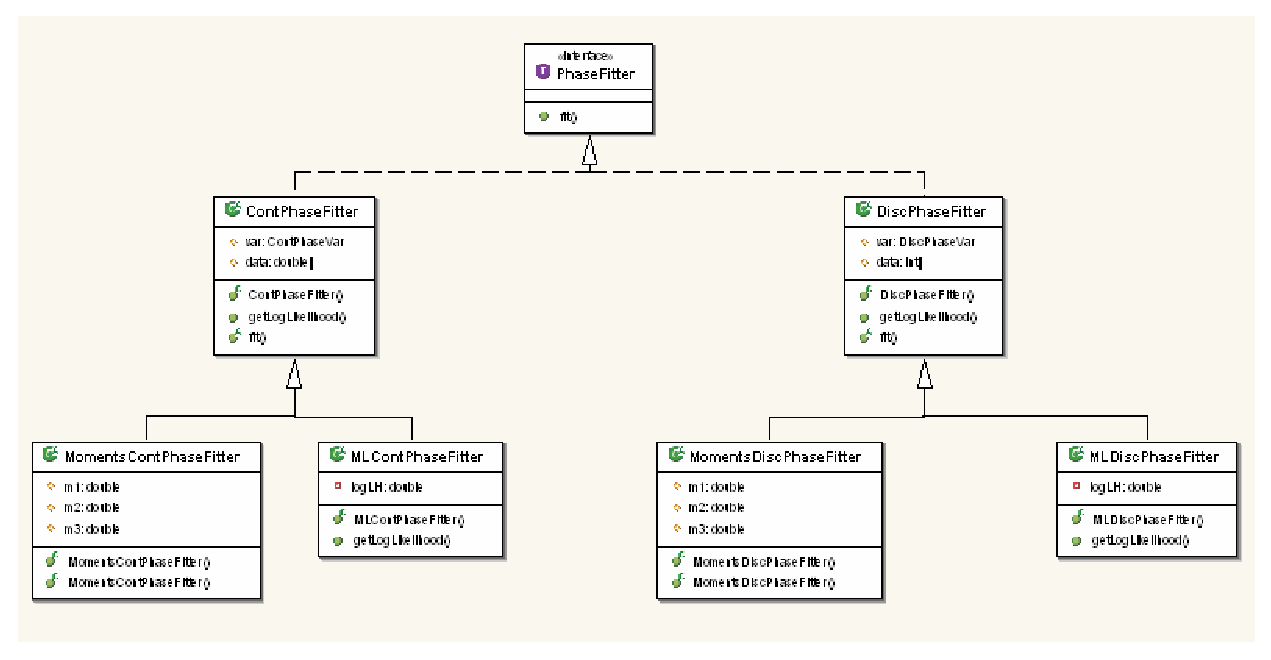
\includegraphics[width=16cm, height=7.5cm]{figs/jphasefit}% height=1.5in
    \caption{Simple \jPhaseFit Package Class Diagram}
    \label{fig:phaseFit}
\end{figure*}

\subsection{Abstract Classes}
In the next level, there are two abstract classes that implement the \texttt{Phase\-Fitter} interface: \texttt{Cont\-Phase\-Fitter} and \texttt{Disc\-Phase\-Fitter}, for the continuous and discrete case, respectively. These classes have two additional issues: a constructor method from a data set in array format; and a method to compute the log-likelihood of the fitted distribution in relation to the data set (\texttt{get\-Log\-likeli\-hood()}). This is done because the log-likelihood is a usual way to compare the performance of fitting algorithms. In addition, these classes specify the continuous or discrete nature of the variable to be fitted in two different ways: the first one is the inclusion of the \texttt{var} attribute, where the fitted variable must be stored (a \texttt{Cont\-Phase\-Var} object for the continuous case or a \texttt{Disc\-Phase\-Var} for the discrete case); the other way is the use of a data array as attribute, that in the continuous case is a double array, and in the discrete case is an integer array.

In the next level of abstract classes, a further division is done between classes that implement Maximum Likeli\-hood (ML) algorithms and those related to Moment Matching techniques. This is done for both continuous and discrete cases. For the ML classes (\texttt{ML\-Cont\-Phase\-Fitter} and \texttt{ML\-Disc\-Phase\-Fitter}), there is a new attribute called \texttt{logLH}, that stores the log-likeli\-hood value in order to take advance of the usual computation of the log-likelihood in the fitting process. For the Moment-Matching related classes (\texttt{Moments\-Cont\-Phase\-Fitter} and \texttt{Moments\-Disc\-Phase\-Fitter}), a new set of attributes is defined: \texttt{m1}, \texttt{m2}, and \texttt{m3}. These are the moments to be matched and are specified with a new constructor that receives only the three moments to be matched. An alternative way is the use of the redefined constructor that receives the data trace and calculates its moments. It must be said that there is not alternative to change the data, moments of log-likelihood attributes from outside the class, implying a safe fitting process.

\subsection{Maximum Likelihood Algorithms}

The set of classes that implement maximum likelihood algorithms are almost all for Continuous PH distributions, because the most of the efforts have been done in that direction. For each one of the following algorithms, there is an associated class that executes the procedures to fit the parameters of a distribution.

\subsubsection{General PH Distribution EM Algorithm}


In 1996 Asmussen, Nerman and Olsson \cite{asmu.nerm.ea96} presented a specialized version of the EM algorithm in order to fit the parameters of the whole set of continuous PH distributions, without reducing the target distribution to a restricted subset. The EM algorithm is a general statistical technique that was first introduced by Dempster et. al. \cite{demp.lair.ea77} to deal with the problem of incomplete data (for a review, see \cite{gour.monf95}). The idea behind this algorithm is that a complete sample from PH realizations should include the selected initial state, the whole path of states followed until absorption, and the time spent in each of these states. With this complete sample, it's easy to estimate the parameters of the distribution.



\subsubsection{Hyper-exponential Distribution EM Algorithm}

The hyper-exponential distribution is a very special case of PH distributions, since the initial probability vector defines the probability of choosing the exponential phase to visit, and the generator matrix have diagonal representation with the rates of the $i$-th phase in the position $(i,i)$. Thus the number of parameter to fit a  $n$-phase hyper-exponential distribution are $2n$. The algorithm proposed by Khayari et. al. \cite{khay.sadr.ea03} is also an EM algorithm like the explained above. It begins with an initial guess of the parameters, that can be random or related to the properties of the trace (e.g. the expected value). The authors propose an easy way to select the initial parameters. Then a function to evaluate the quality of the parameters is calculated in the E-step through the probability density function of the data trace given the parameters. In the M-step, the new set of parameters is computed using estimators for the rates and the probabilities but not for the number of phases, that is taken as a given parameter.



\subsubsection{Hyper-Erlang Distribution EM Algorithm}

In 2005, Th�mmler et. al. presented a method that fits the parameters of a hyper-Erlang distribution \cite{thum.buch.ea05}, which is a very interesting subset of the PH distributions since they are also dense in $[0,\infty)$. In some results provided by them, the EM algorithm developed for this special class has a better behavior in terms of likelihood than the one designed for the complete Phase family \cite{asmu.nerm.ea96}. The algorithm receives as a parameter the number of Erlang branches in the distribution as well as the total number of exponential phases in the distribution. With this information, the algorithm determines all the possible configurations of the Erlang branches and executes a version of the EM algorithm for each case. Finally, the configuration with the greatest likelihood is selected as the result of the algorithm. 

\subsection{Moment Matching Algorithms}

The distribution moments usually play an important role in the performance analysis of real systems \cite{osog.harc06}. This has been an important motivation for the improvement of moment matching techniques, and the attention given by different research communities (Operations Research, Computer Science and Telecommunication Networks, among others). Some of the most recent advances have been implemented in the jPhaseFit module, as will be explained in this section.

\subsubsection{Acyclic Continuous order-2 Distributions}

In 2002 Telek and Heindl \cite{tele.hein02} proposed an algorithm to fit the parameters of an acyclic PH distributions of second order (two phases). Acyclic distributions have been extensively studied since they have some important properties, as a canonic form developed by Cumani \cite{cuma82} and an upper triangular transition or generator matrix. In that paper, they establish bounds on the set of first three moments representable by acyclic distributions of second order, for the discrete and continuous cases. Over the characterization of these bounds, they build the algorithm that matches three moments with the three parameters of this distribution: the rates of each phase and the absorption probability after the first phase (the initial probability is all in the first phase as in the Coxian distribution).



\subsubsection{Erlang-Coxian Distributions}
The next step in moment-matching techniques was given by Osogami and Harchol in a series of papers \cite{osog.harc03, osog.harc03b, osog.harc06}. This extension consists on the characterization of the bounds imposed over the first three moments representable by a PH distribution with $n$ phases. They also introduce Erlang-Coxian distributions, named because they can be represented as the convolution of an Erlang and a Coxian distribution of second order. They present an algorithm to fit the parameters of a Erlang-Coxian distribution with or without mass at zero, an important issue in constructing matrix-geometric models from phase type distributions. An important issue is that the algorithm itself determines the number of phases needed to represent the set of moments, making easier the use of the algorithm since the user doesn't need to try with different configurations. The resulting distributions are not large in the number of phases but are not strictly minimal.


\subsubsection{Acyclic Continuous Distributions}

One of the most recent effort done in this area was made in 2005 by Bobbio, Horvath and Telek \cite{bobb.horv.ea05}, who present an algorithm to match a set of first three moments with acyclic PH distributions (APH). They show the possible sets that can be represented by an acyclic distribution of order $n$. Then they show how to match the first three moments in a minimal way, i.e. using the minimal number of phases needed to do it. It is done by determining the region representable by an APH of $n$ phases but not with an APH with $n-1$. This region is then partitioned in five areas that represent different distribution configurations, such as the Erlang-Exp structure that represents and $n-1$ Erlang distribution with an additional exponential phase after it.

The algorithm proposed by the authors for the positive case is implemented in the \texttt{MomentsACPHFit} class. There the algorithm begins with the first three non-central moments and computes the first two normalized moments. With this information, the required number of phases is computed and the moment set is evaluated in order to find in which region it falls. When it is determined, the parameters are fitted according to the equations presented by the authors.

\subsection{\jPhaseFit Examples}

In order to illustrate the use of \jPhaseFit, two examples are given in this section. The first one is shown in Figure \ref{fig:ex31}, where the first step is the loading of a data set that comes from a text file. The data set is stored in an array of doubles and it is used as the parameter to create the \texttt{fitter} object. This fitter is of the \texttt{EMHyperErlangfFit} type, that implements the method proposed in \cite{thum.buch.ea05}. After the fitter initialization, a PH variable ($V_1$) is created as the result of fitting procedure applied over the data set, and the specification of the number of phases desired for the fitted distribution (4). Finally, the parameters of the fitted variable are printed, as well as the log-likelihood reached by the method in the last iteration. The result is shown in Figure \ref{fig:resEx31}.

\begin{figure}[htbp]
	\centering
	\lstinclude{figs/example31.java}
	\caption{\jPhaseFit: Example 1}
	\label{fig:ex31}
\end{figure}

\begin{figure}[htbp]
	\centering
	\lstinclude{figs/resExample31.txt}
	\caption{\jPhaseFit: Result for Example 1}
	\label{fig:resEx31}
\end{figure}



The next example is shown in Figure \ref{fig:ex32}. It shows the creation of a \texttt{fitter} of the \texttt{Moments\-ACPH\-Fit} type, which implements the algorithm proposed in \cite{bobb.horv.ea05}. This \texttt{fitter} is created by specifying a set of moments that the fitted variable should have, in this case $m_1=2$, $m_2=6$ and $m_3=25$. As this information is enough for the method, it is not necessary to specify any other parameter and the variable $V_1$ is created as the fitted variable coming from running the method for the moments set. Finally, the variable is printed, as well as its moments, which naturally correspond to the asked ones. This result is shown in Figure \ref{fig:resEx32}.

\begin{figure}[htbp]
	\centering
	\lstinclude{figs/example32.java}
	\caption{\jPhaseFit: Example 2}
	\label{fig:ex32}
\end{figure}




\begin{figure}[htbp]
	\centering
	\lstinclude{figs/resExample32.txt}
	\caption{\jPhaseFit: Result for Example 2}
	\label{fig:resEx32}
\end{figure}


\newpage
%\section{A final Example}


\printindex

%\bibliographystyle{plain}
\bibliographystyle{siam}
%\bibliography{fernandoMaestria-bib}
%\bibliographystyle{uniandes-tesis}
%\bibliographystyle{article} %
%\addcontentsline{toc}{section}{References}
\bibliography{%
../../Biblio/Optimization,%
../../Biblio/Transportation,%
../../Biblio/ComputerScience,%
../../Biblio/Riano,%
../../Biblio/Manufacturing,%
../../Biblio/Stochastics,%
../../Biblio/Math}


\end{document}
